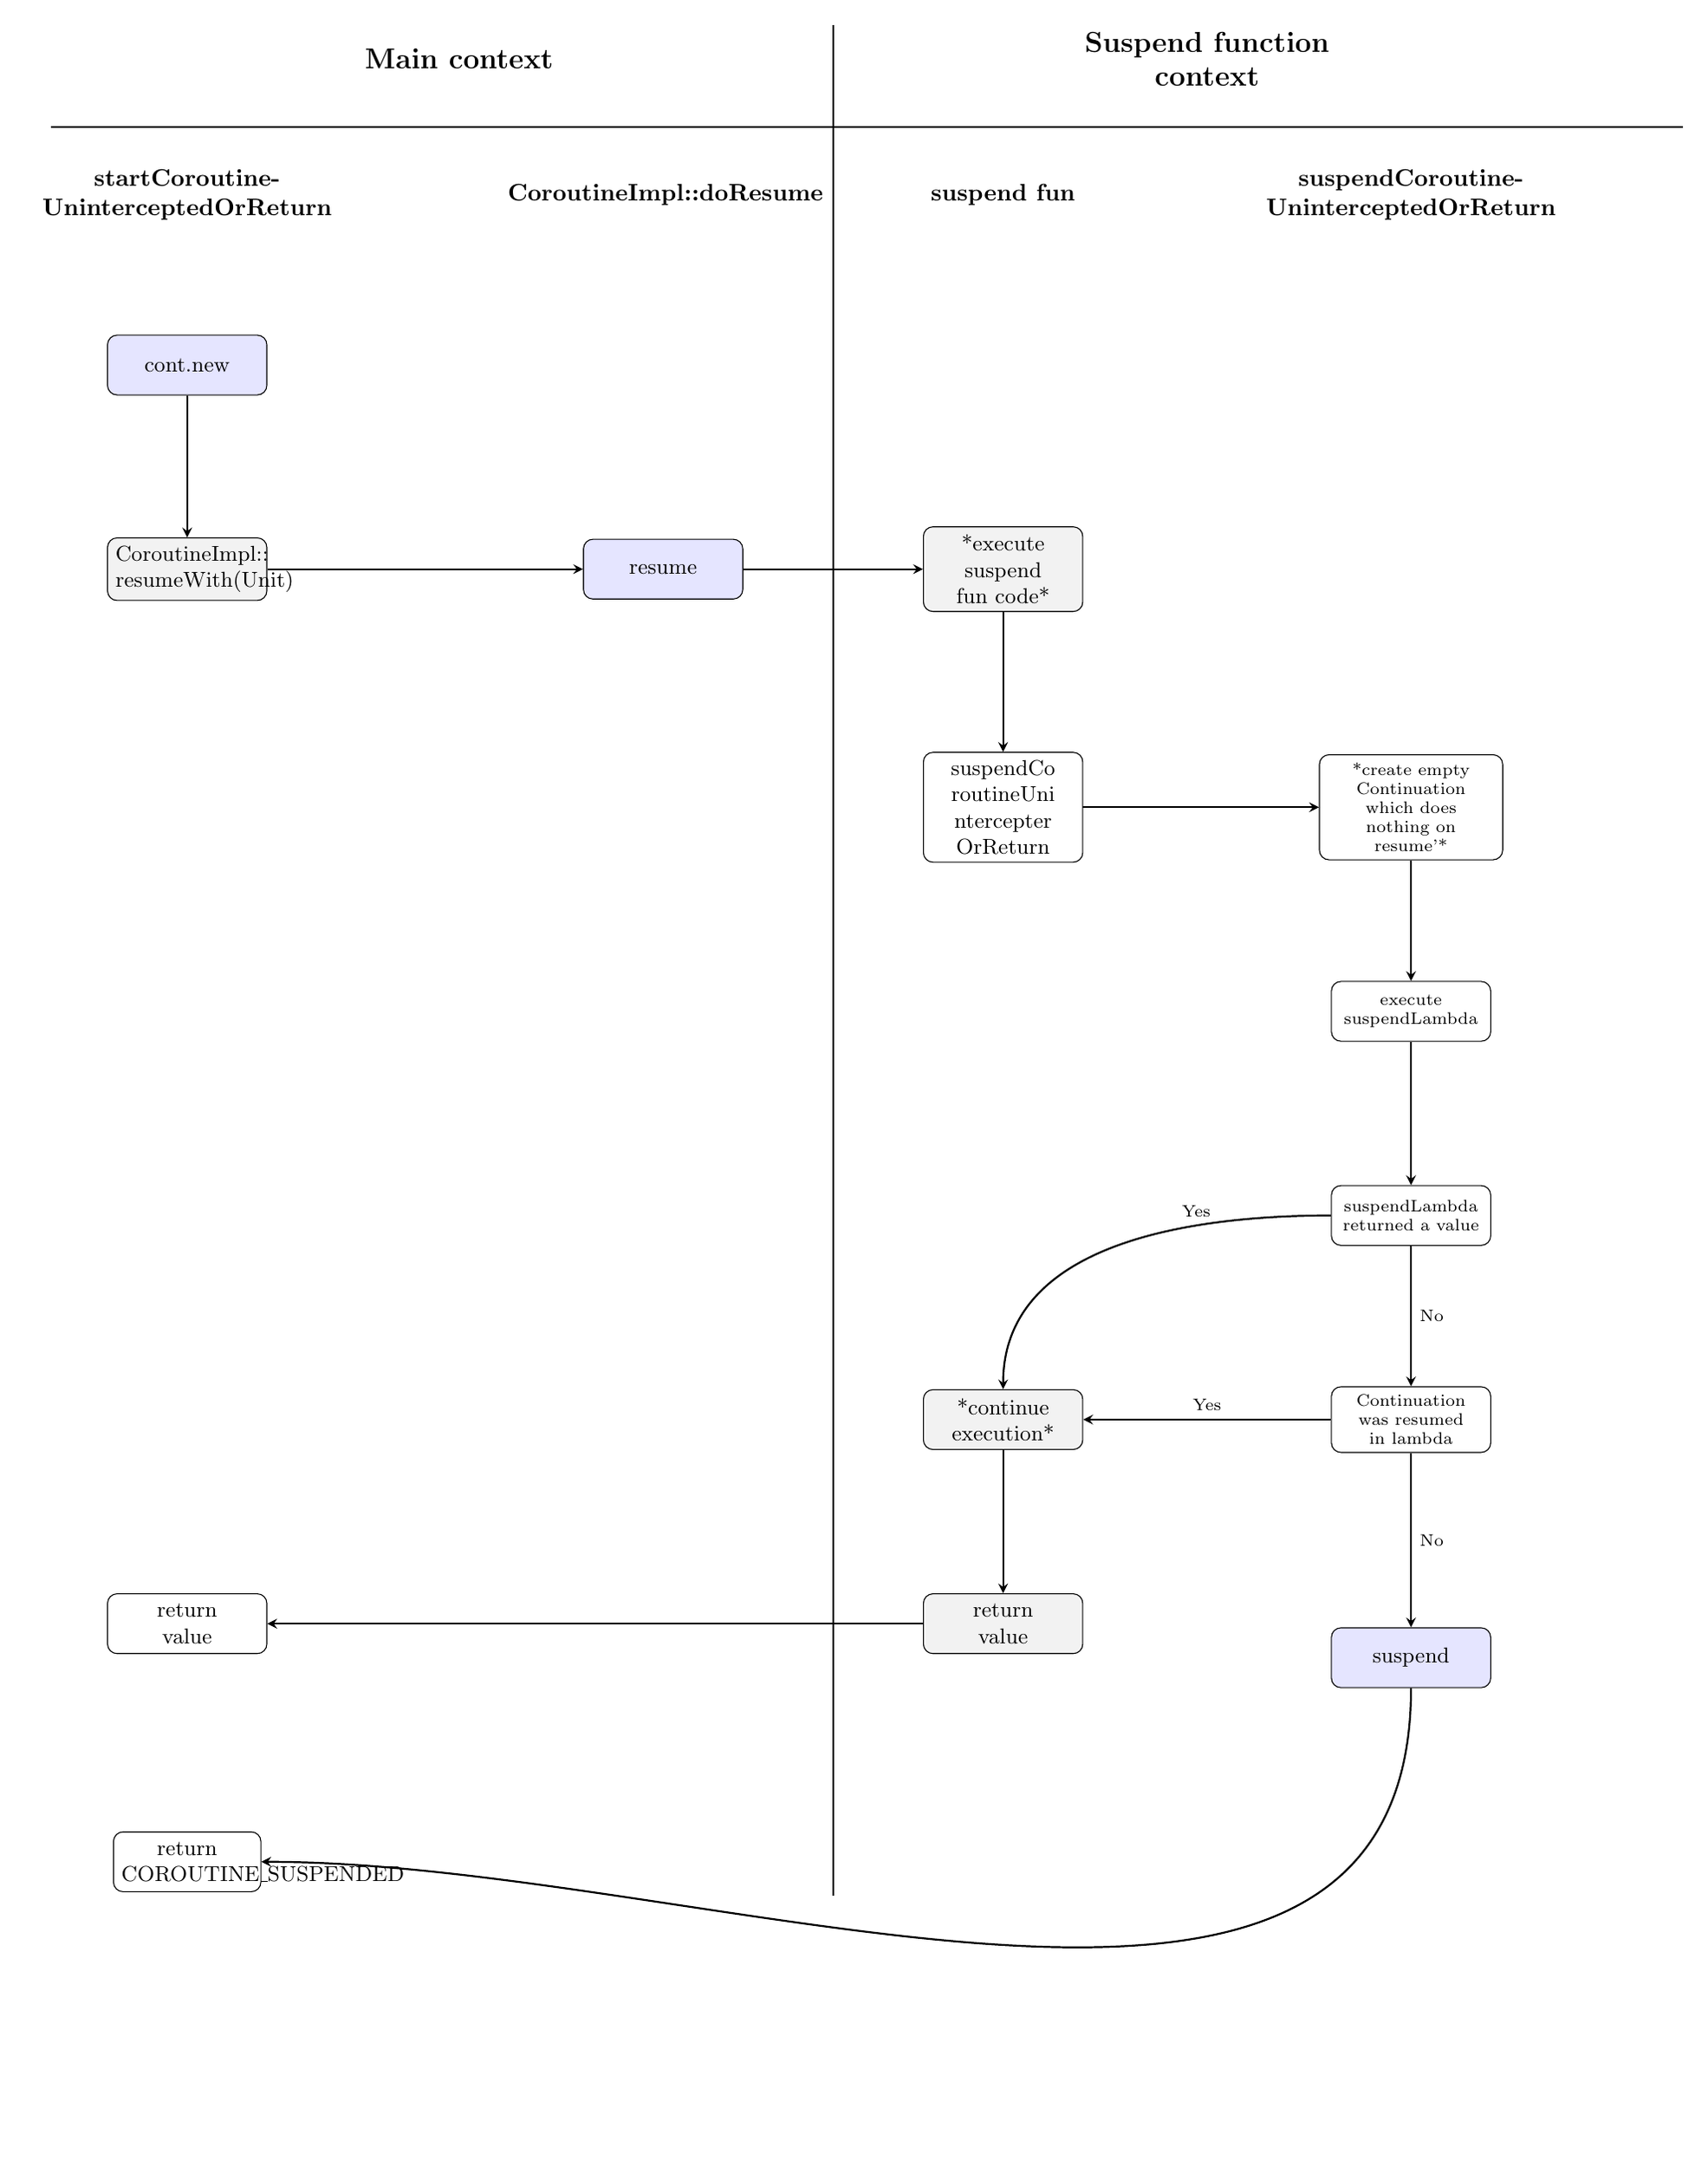
\begin{tikzpicture}[
    node distance=1.2cm and 3cm,
    every node/.style={font=\small},
    block/.style={rectangle, draw, fill=blue!10, text width=6em, text centered, rounded corners, minimum height=2.5em},
    decision/.style={diamond, draw, fill=yellow!10, text width=5em, text centered, aspect=2, inner sep=1pt},
    action/.style={rectangle, draw, fill=green!10, text width=7em, text centered, rounded corners, minimum height=2.5em},
    suspend/.style={rectangle, draw, fill=orange!20, text width=7em, text centered, rounded corners, minimum height=2.5em},
    title/.style={font=\large\bfseries, text width=13em, align=center},
    subtitle/.style={font=\normalsize\bfseries, text width=10em, align=center},
    whiteNote/.style={rectangle, draw, fill=white, text width=6em, text centered, rounded corners, minimum height=2.5em},
    blueNote/.style={rectangle, draw, fill=blue!10, text width=6em, text centered, rounded corners, minimum height=2.5em},
    yellowNote/.style={rectangle, draw, fill=gray!10, text width=6em, text centered, rounded corners, minimum height=2.5em},
    arrow/.style={->, >=stealth, thick},
    transfer/.style={->, >=stealth, thick},
    solidarrow/.style={->, >=stealth, thick},
    label/.style={font=\scriptsize, text=black}
]

% -------------------------
% Main Dividers
% -------------------------
    \draw[thick] (-2, 0) -- (22, 0); % Horizontal line
    \draw[thick] (9.5, 1.5) -- (9.5, -26); % Vertical line

% -------------------------
% Headers & Subheaders
% -------------------------
    \node[title] at (4, 1) {Main context};
    \node[title] at (15, 1) {Suspend function\\context};

    \node[subtitle, text width=13em] (sub1) at (0, -1) {startCoroutine-\\UninterceptedOrReturn};
    \node[subtitle, text width=13em] (sub2) at (7, -1) {CoroutineImpl::doResume};
    \node[subtitle] (sub3) at (12, -1) {suspend fun};
    \node[subtitle, text width=13em] (sub4) at (18, -1) {suspendCoroutine-\\UninterceptedOrReturn};

% -------------------------
% Nodes - Column 1 (X=0)
% -------------------------
    \node[blueNote] (n1_1) at (0, -3.5) {cont.new};
    \node[yellowNote] (n1_2) at (0, -6.5) {CoroutineImpl::\\resumeWith(Unit)};
    \node[whiteNote] (n1_3) at (0, -22) {return\\value};
    \node[whiteNote, text width=5.5em] (n1_4) at (0, -25.5) {return\\COROUTINE\_SUSPENDED};

% -------------------------
% Nodes - Column 2 (X=7)
% -------------------------
    \node[blueNote] (n2_1) at (7, -6.5) {resume};

% -------------------------
% Nodes - Column 3 (X=12)
% -------------------------
    \node[yellowNote] (n3_1) at (12, -6.5) {*execute\\suspend\\fun code*};
    \node[whiteNote, text width=6em] (n3_2) at (12, -10) {suspendCo\\routineUni\\ntercepter\\OrReturn};
    \node[yellowNote] (n3_3) at (12, -19) {*continue\\execution*};
    \node[yellowNote] (n3_4) at (12, -22) {return\\value};

% -------------------------
% Nodes - Column 4 (X=18)
% -------------------------
    \node[whiteNote, font=\scriptsize, text width=7em] (n4_1) at (18, -10) {*create empty\\Continuation\\which does\\nothing on\\resume'*};
    \node[whiteNote, font=\scriptsize] (n4_2) at (18, -13) {execute\\suspendLambda};
    \node[whiteNote, font=\scriptsize] (n4_3) at (18, -16) {suspendLambda\\returned a value};
    \node[whiteNote, font=\scriptsize] (n4_4) at (18, -19) {Continuation\\was resumed\\in lambda};
    \node[blueNote] (n4_5) at (18, -22.5) {suspend};

% -------------------------
% Arrows & Routing
% -------------------------
    % Downward & Rightward Top Flow
    \draw[arrow] (n1_1) -- (n1_2);
    \draw[arrow] (n1_2) -- (n2_1);
    \draw[arrow] (n2_1) -- (n3_1);
    \draw[arrow] (n3_1) -- (n3_2);
    \draw[arrow] (n3_2) -- (n4_1);
    \draw[arrow] (n4_1) -- (n4_2);
    \draw[arrow] (n4_2) -- (n4_3);

    % Yes/No Branching from "suspendLambda returned a value"
    % 'Yes' branch curves left and down, with a small dot marker
    \draw[arrow] (n4_3.west) to[out=180, in=90]
    node[above, font=\scriptsize, pos=0.3] {Yes} (n3_3.north);

    % 'No' branch goes straight down
    \draw[arrow] (n4_3.south) -- node[right, font=\scriptsize] {No} (n4_4.north);

    % Yes/No Branching from "Continuation was resumed"
    % 'Yes' branch goes straight left, with a small dot marker
    \draw[arrow] (n4_4.west) --
    node[above, font=\scriptsize] {Yes} (n3_3.east);

    % 'No' branch goes straight down
    \draw[arrow] (n4_4.south) -- node[right, font=\scriptsize] {No} (n4_5.north);

    % Bottom Flow - Values and Suspensions
    \draw[arrow] (n3_3) -- (n3_4);

    % Return value straight back to main context
    \draw[arrow] (n3_4) -- (n1_3);

    % Suspend path routes down, then horizontally across back to main context
    \draw[arrow] (n4_5.south) to[out=270, in=0] (n1_4.east);
\end{tikzpicture}
